\begin{problem}{울타리}
	{standard input}{standard output}
	{1초}{256MB}{}
	
	JOI 씨는 IOI 나라의 거대한 토지를 소유하고 있다. IOI 나라의 토지는 좌표평면으로 표현되며, 직교하는 X축과 Y축이 정해져 있다. X 좌표가 $x$, Y 좌표가 $y$인 점을 $(x, y)$로 표현한다. JOI 씨가 소유하고 있는 토지는 X 좌표와 Y 좌표 모두 $-10^{100}$ 이상 $10^{100}$ 이하인 영역이다. 이 토지에서 X 좌표와 Y 좌표 모두 $-S$ 이상 $S$ 이하인 영역은 목초지이며, 소를 기르고 있다.
	
	JOI 씨는 소가 도망가지 않도록 목초지를 몇 개의 울타리로 감싸기로 했다. 울타리는 길이가 양의 실수인 선분으로 표현된다. 여기서 목초지를 울타리로 감싼다는 것은, 목초지 내부의 어떤 점에서부터도 울타리가 존재하는 지점 (울타리의 경계도 포함한다) 을 지나지 않고 JOI 씨의 토지 밖으로 나가는 것이 불가능하다는 것을 의미한다. JOI 씨의 토지에는 처음에 몇 개의 울타리가 놓여있으므로 이 울타리를 사용하여 목초지를 감싸도 된다. 처음에 존재하는 어떤 두 울타리에 대해 이 두 울타리의 공통점이 존재한다면, 이 점은 적어도 한 울타리의 끝점이다.
	
	JOI 씨는 울타리를 새로 몇 개 배치하기로 했다. 이때, 목초지의 내부나 JOI 씨의 토지의 이외를 지나도록 울타리를 배치하는 것은 불가능하지만, 목초지의 경계에 배치하는 것은 상관없다. 이 조건을 만족하면 어떤 길이의 울타리를 어떤 방향으로 배치해도 상관없다. 길이 $l$의 ($l > 0$) 울타리를 한 개 추가하는 데에는 비용이 $l$만큼 든다. 여기서 울타리끼리 교차하거나, 울타리의 끝점이 다른 끝점과 일치해도 상관없다. 또한, 울타리의 끝점이 다른 울타리에 포함되어 있어도 상관없다.
	
	JOI 씨는 가능한 한 적은 비용으로 목초지를 울타리로 감싸려고 한다.
	
	JOI 씨의 목초지의 크기와 처음 놓여있는 울타리의 정보가 주어졌을 때, 목초지를 울타리로 감싸는 데 필요한 비용의 최솟값을 구하는 프로그램을 작성하여라.
	
	
	\InputFile
	
	표준 입력에서 다음 입력이 주어진다.
	
	\begin{itemize}
		\item 첫째 줄에는 두 개의 정수 $N$, $S$가 공백으로 구분되어 주어진다. 이는 토지에서 X 좌표와 Y 좌표 모두 $-S$ 이상 $S$ 이하인 영역은 목초지이며, JOI 씨가 소유하고 있는 토지에 처음에 $N$ 개의 울타리가 놓여있다는 것을 의미한다.
		\item 다음 $N$ 개의 줄의 $i$ 번째 ($1 \le i \le N-1$) 줄에는 네 개의 정수 $A_i$, $B_i$, $C_i$, $D_i$가 공백으로 구분되어 주어진다. 이는 $i$ 번째 울타리가 두 개의 선분 $(A_i, B_i)$와 $(C_i, D_i)$를 잇는 선분이라는 것을 의미한다.
	\end{itemize}
		
	\OutputFile
	
	목초지를 울타리로 감싸는 데 필요한 비용의 최솟값을 첫째 줄에 출력하여라. 출력하는 소수점 이하의 개수에 제한은 없지만, 답과의 절대오차가 0.01 이하여야 한다.
	
	\Constraints
	
	\begin{itemize}
		\item $1 \le N \le 100$.
		\item $1 \le S \le 200$.
		\item $-200 \le A_i \le 200$ ($1 \le i \le N$).
		\item $-200 \le B_i \le 200$ ($1 \le i \le N$).
		\item $-200 \le C_i \le 200$ ($1 \le i \le N$).
		\item $-200 \le D_i \le 200$ ($1 \le i \le N$).
		\item $(A_i, B_i) \ne (C_i, D_i)$ ($1 \le i \le N$).
		\item 입력으로 주어지는 울타리는 목초지의 내부를 지나지 않는다.
		\item 입력으로 주어지는 서로 다른 두 울타리에 대해 이 두 울타리의 공통점이 존재한다면, 이 점은 적어도 한 울타리의 끝점이다.
	\end{itemize}
	
	
	\SubtaskWithCost{1}{18}
	\begin{itemize}
		\item $N = 1$.
	\end{itemize}

	\SubtaskWithCost{2}{33}
	\begin{itemize}
		\item $N \le 6$.
	\end{itemize}
	

	\SubtaskWithCost{3}{49}
	추가 제한조건이 없다.
	
	\Examples
	
	\begin{example}
		\exmp{
			3 4
			-3 5 1 8
			-4 3 -4 6
			5 1 7 2
		}{%
			29.0000000000
		}%
	\end{example}
	
	이 입력 예제에서는 처음에 왼쪽 아래의 지도처럼 울타리가 배치되어 있다. 중앙에 점선으로 표시된 정사각형은 목초지의 외곽이다.
	
	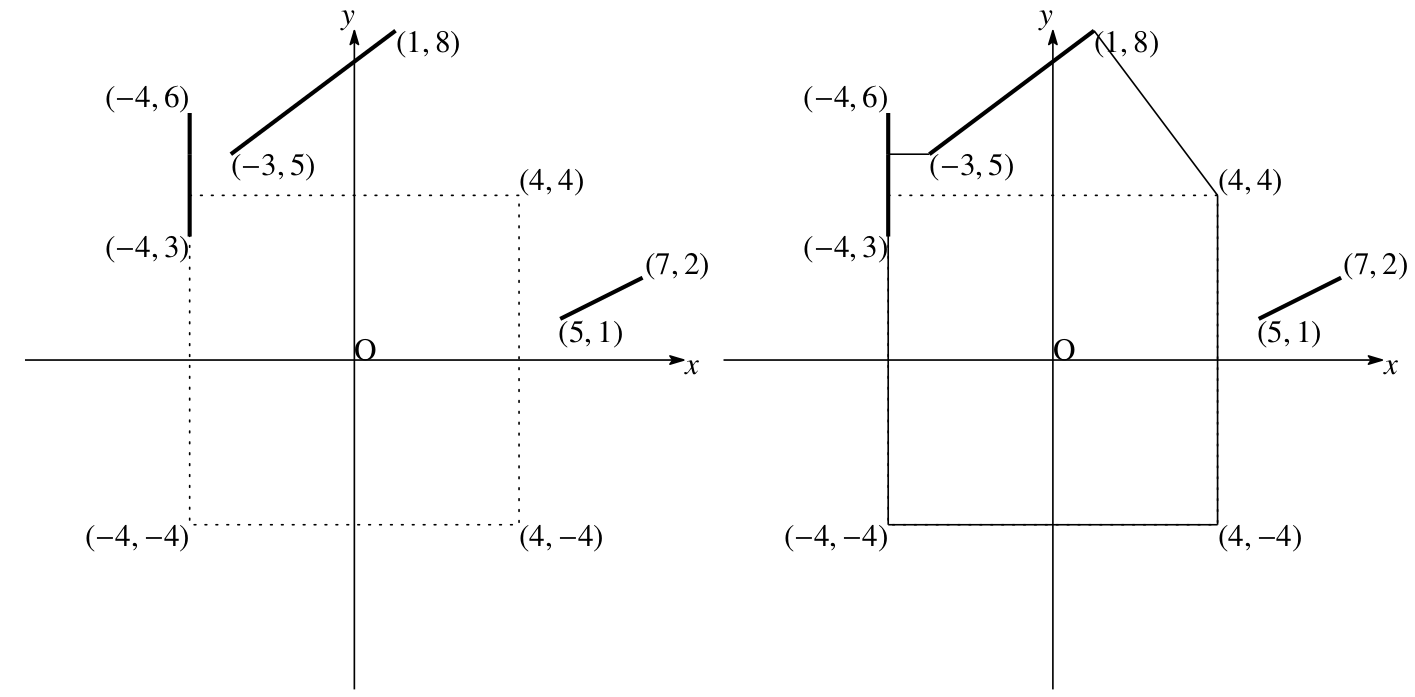
\includegraphics[width=\linewidth]{img1.png}
	
	오른쪽 아래의 실선으로 표시된 새로운 울타리를 배치하면 목초지를 감쌀 수 있다. 이때, 비용은 29이고 최소이다. 즉, 이 입력 예제의 경우 \texttt{29.0000000000} 이외에도 \texttt{29}나 \texttt{28.999}를 출력해도 정답으로 판정한다.
	
	\begin{example}
		\exmp{
1 2
-3 -3 -3 -2
}{%
16.0000000000
}%
	\end{example}

	처음에 배치된 울타리를 사용하지 않고 목초지를 울타리로 감쌀 수 있다는 것에 유의하여라.

	\begin{example}
	\exmp{
		4 3
		4 -1 3 4
		-4 2 -2 4
		-4 0 -5 6
		0 -6 5 -2
	}{%
		14.1392801789
	}%
	\exmp{
		10 80
		175 95 60 -146
		-106 57 18 185
		190 -68 177 -142
		84 -195 127 -179
		34 143 126 69
		-92 133 -190 80
		-157 -66 -119 -161
		-85 -124 129 -171
		141 181 175 175
		107 -38 150 148
	}{%
	238.4778364511
	}%
\end{example}

	
	
\end{problem}

